\documentclass[]{beamer}
%\usepackage[MeX]{polski}
%\usepackage[cp1250]{inputenc}
\usepackage{polski}
\usepackage[utf8]{inputenc}
\beamersetaveragebackground{blue!10}
\usetheme{Warsaw}
\usecolortheme[rgb={0.1,0.5,0.7}]{structure}
\usepackage{beamerthemesplit}
\usepackage{multirow}
\usepackage{multicol}
\usepackage{array}
\usepackage{graphicx}
\usepackage{enumerate}
\usepackage{amsmath} %pakiet matematyczny
\usepackage{amssymb} %pakiet dodatkowych symboli

\title{CHELSEA FOOTBALL CLUB}
\date{}

\begin{document}

\frame
{
	\centering
	
\includegraphics[width=0.4\textwidth]{logo.png}
	\maketitle	
}
\frame
{
	\frametitle{Historia}
	\begin{block}
		{Powstanie}
		W 1904 stadion Stamford Bridge został nabyty przez przedsiębiorców budowlanych Henry Augustusa i Josepha T. Mearsów. Dostosowali oni obiekt do potrzeb gry w piłkę nożną i zamierzali sprzedać klubowi Fulham F.C. Oferta kupna została jednak odrzucona, dlatego biznesmeni postanowili założyć klub. Dokonano tego 14 marca 1905 w pubie „The Rinsing Sun”, a klub otrzymał nazwę sąsiedniej dzielnicy – Chelsea. Pierwszy oficjalny sezon zespół rozpoczął rok później w drugiej lidze pod opieką trenera Johna Robertsona. Pierwszym oficjalnym spotkaniem był przegrany 0:1 mecz ze Stockport County F.C., który odbył się 1 września 1905r. Historyczny, pierwszy rekord frekwencji padł w Wielki Piątek w 1906 roku, podczas meczu z Manchester United F.C., który obejrzało na Stamford Bridge 67 tysięcy widzów.
	\end{block}
	%\begin{exampleblock}
		%{To jest przykład}
		%\texttt{for(int i=0;i<n;i++)
		%		cout<<"Hello world!";}
%	\end{exampleblock}
	%\begin{alertblock}
		%{Uwaga!}
		%Tu wpisujemy tekst, który wymaga podkreślenia.
	%\end{alertblock}
}
\frame
{
	\frametitle{Historia herbu}
	\begin{block}
		{Na przestrzeni lat Chelsea miała 5 różnych herbów}
		\centering
		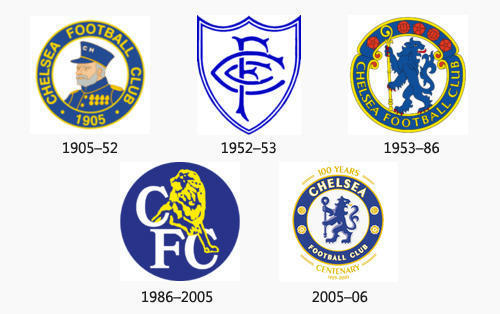
\includegraphics[width=0.7\textwidth]{logos.jpg}
	\end{block}
}
\frame
{
	\frametitle{Stroje}
	\begin{block}
		{Oto pełny zestaw strojów na sezon 2017/18}
		\centering
		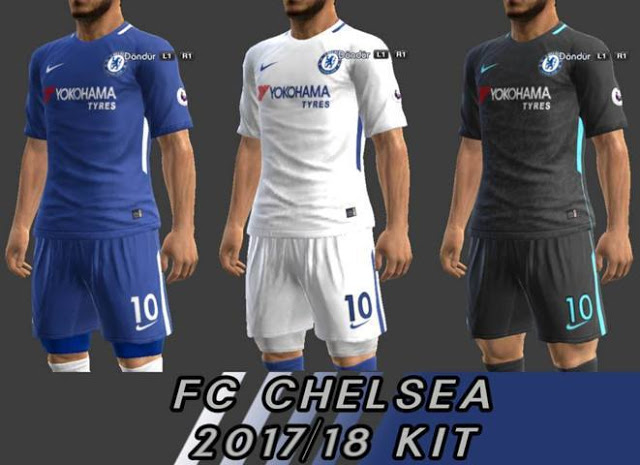
\includegraphics[width=0.7\textwidth]{kits.jpg}
	\end{block}
}
\frame
{
	\frametitle{Stadion}
	\begin{block}
		{Tak prezentuje się stadion drużyny - Stamford Bridge w Londynie}
		\centering
		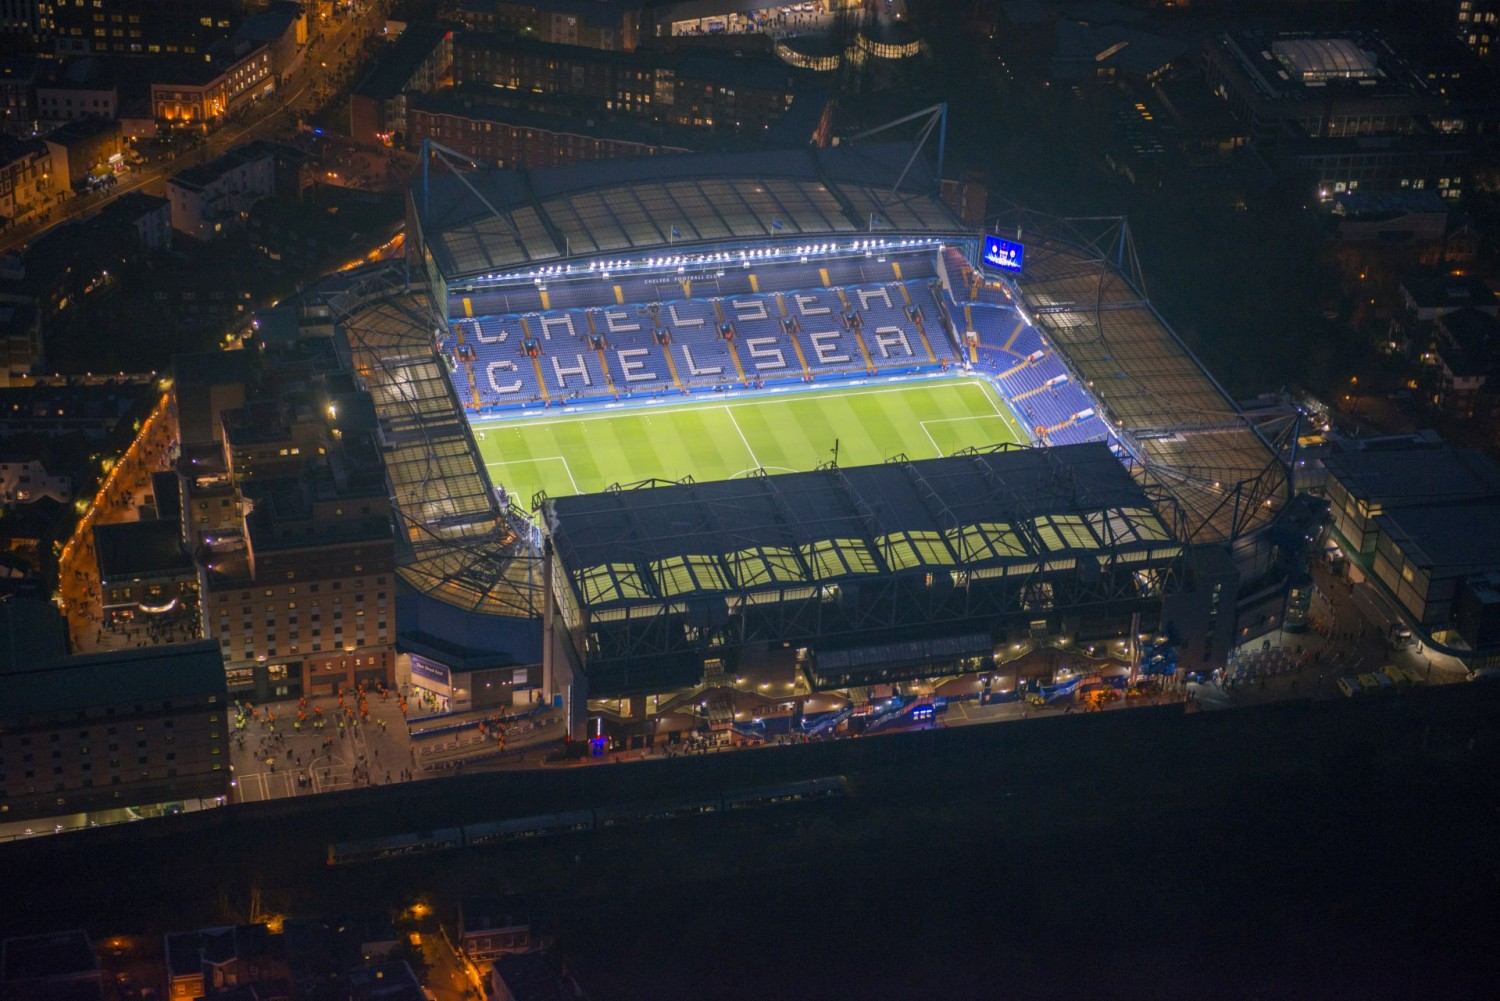
\includegraphics[width=0.8\textwidth]{sb.jpg}
	\end{block}
}
\frame
{
	\frametitle{Skład}
	\begin{block}
		{Tak prezentuje się formacja drużyny na sezon 2017/18}
		\centering
		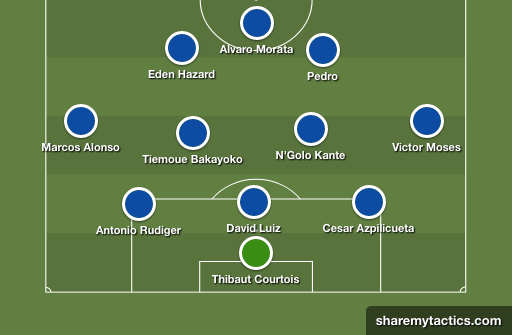
\includegraphics[width=0.8\textwidth]{squad.png}
	\end{block}
}
\frame
{
	\frametitle{Sukcesy}
	\begin{block}
		{Ostatnie sukcesy drużyny:}
		\centering
		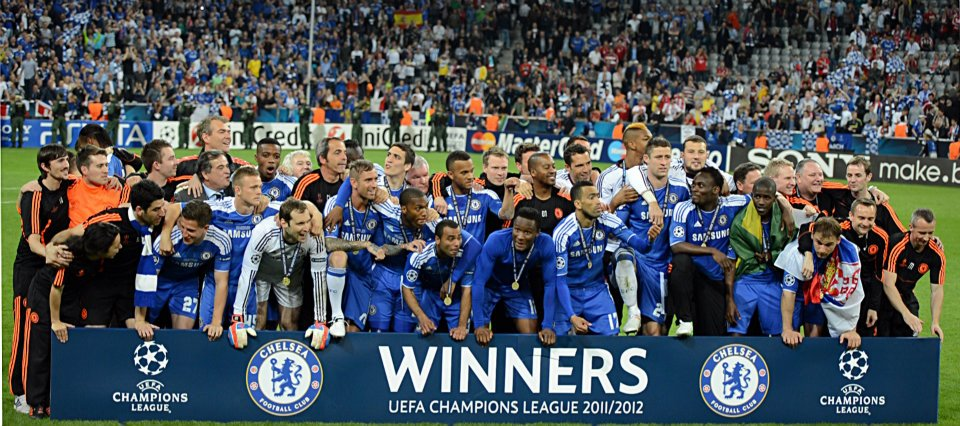
\includegraphics[width=1\textwidth]{cl.jpg}
		\newline Puchar Ligi Mistrzów w sezonie 2011/12
	\end{block}
}
\frame
{
	\frametitle{Sukcesy}
	\begin{block}
		{Ostatnie sukcesy drużyny:}
		\centering
		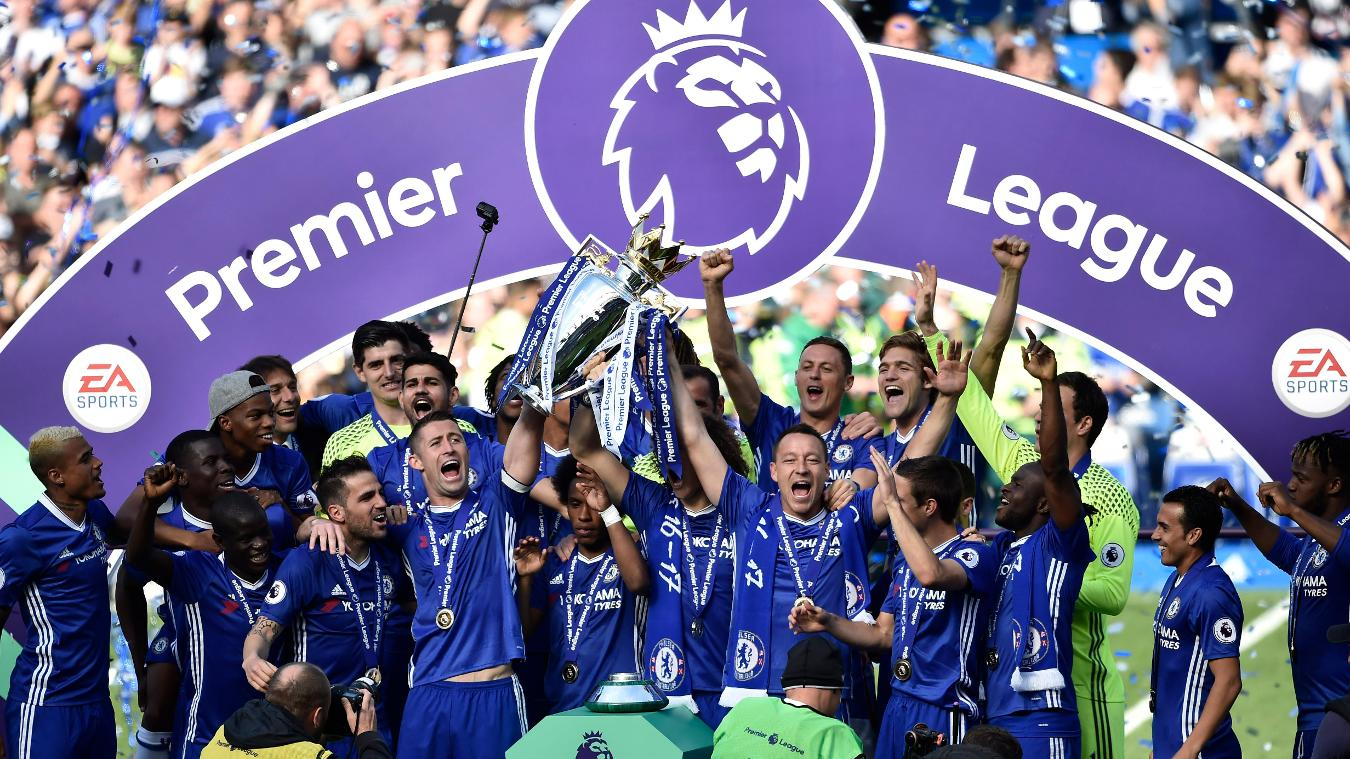
\includegraphics[width=1\textwidth]{pl.jpg}
		\newline Mistrzostwo Anglii w sezonie 2016/17
	\end{block}
}
\frame
{
	\frametitle{Współczesne legendy drużyny}
	\begin{block}
		{John Terry, nr 26}
		\centering
		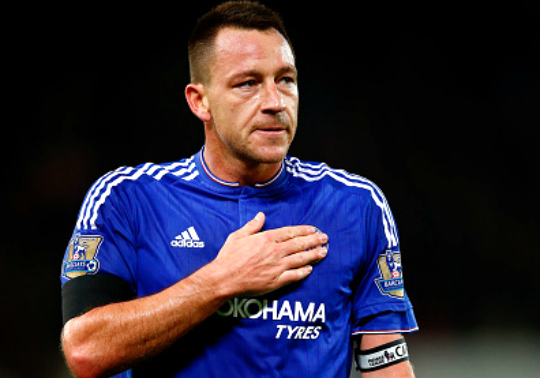
\includegraphics[width=0.8\textwidth]{jt.jpg}
	\end{block}
}
\frame
{
	\frametitle{Współczesne legendy drużyny}
	\begin{block}
		{Frank Lampard, nr 8}
		\centering
		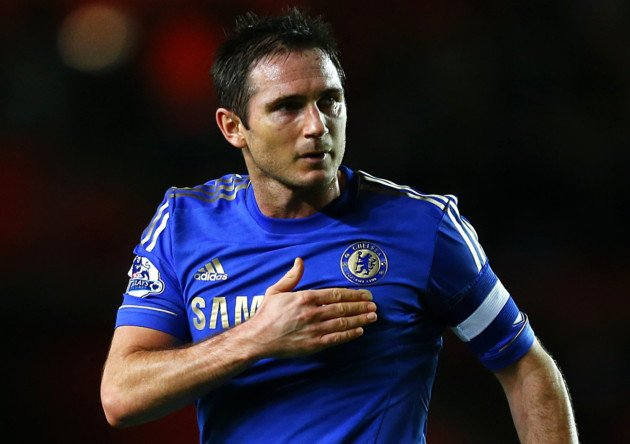
\includegraphics[width=0.8\textwidth]{fl.jpg}
	\end{block}
}
\frame
{
	\frametitle{Współczesne legendy drużyny}
	\begin{block}
		{Didier Drogba, nr 11}
		\centering
		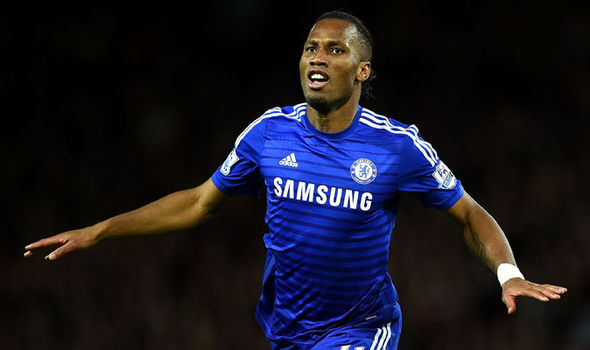
\includegraphics[width=1\textwidth]{dd.jpg}
	\end{block}
}
\end{document}